% =============================================================================
%  ch82_cyclic_validation.tex — Progressive cyclic validation of FE² pipeline
% =============================================================================

\chapter{Progressive Cyclic Validation of the FE² Pipeline}
\label{ch:cyclic-validation}

This chapter documents a progressive validation suite for the
nonlinear analysis and FE² multiscale pipeline.  Five cases of
increasing complexity are solved under the same cyclic displacement
protocol, using a ``4-legged table'' geometry as the base
structure.  Beyond presenting the numerical results, the chapter
devotes particular attention to three aspects discovered during the
validation campaign: (i)~implementation bugs that affected the
sub-model solver, (ii)~the root-cause analysis of the two-way
coupling failure, and (iii)~a detailed cross-reference between the
Ko--Bathe concrete model article and the \texttt{KoBatheConcrete3D}
implementation, including the derivation and implementation of a
numerically consistent tangent.


%----------------------------------------------------------------------
\section{Motivation}
\label{sec:cyclic-motivation}

The seismic table analysis of Chapter~\ref{ch:table-multiscale}
demonstrated the full FE² pipeline but posed challenges in isolating
the source of convergence difficulties.  This validation suite
replaces the dynamic seismic excitation with a quasi-static
displacement-controlled cyclic protocol, guaranteeing that each
amplitude level is reached regardless of dynamic effects.  The
progressive structure isolates complexity layer by layer:

\begin{enumerate}
  \item \textbf{Case~1} — Single beam element with RC fiber sections,
    validating the constitutive response at the section level.
  \item \textbf{Case~2} — Single continuum column with KoBathe
    concrete and embedded rebar, validating the 3D constitutive model.
  \item \textbf{Case~3} — Full table structural model (4~beams +
    MITC16 shell), validating the mixed beam--shell nonlinear solver.
  \item \textbf{Case~4} --- Table with FE² sub-models, one-way
    coupling (macro $\to$ micro only).
  \item \textbf{Case~5} --- Table with FE² sub-models, two-way
    staggered coupling (macro $\leftrightarrow$ micro).
\end{enumerate}


%----------------------------------------------------------------------
\section{Shared Geometry and Material Properties}
\label{sec:cyclic-geometry}

All cases share the same RC column section and material parameters,
matching the table geometry of Chapter~\ref{ch:table-multiscale}:

\begin{table}[htbp]
\centering
\caption{Shared geometric and material parameters.}
\label{tab:cyclic-params}
\begin{tabular}{lrl}
\toprule
\textbf{Parameter}    & \textbf{Value} & \textbf{Unit} \\
\midrule
Plan dimensions       & $5.0 \times 5.0$ & m \\
Column height $H$     & 3.2        & m \\
Column section        & $0.25 \times 0.25$ & m \\
Clear cover           & 0.03       & m \\
Bar diameter          & 16         & mm \\
$f'_c$                & 30.0       & MPa \\
$E_s$                 & 200\,000   & MPa \\
$f_y$                 & 420        & MPa \\
$b$ (hardening)       & 0.01       & --- \\
Slab thickness        & 0.20       & m \\
\bottomrule
\end{tabular}
\end{table}


%----------------------------------------------------------------------
\section{Cyclic Displacement Protocol}
\label{sec:cyclic-protocol}

The loading protocol is a triangular cyclic displacement with four
amplitude levels:

\[
  \delta_k \in \{1, 2, 4, 8\} \times \delta_y
  \qquad \text{where } \delta_y \approx 0.01 \text{ m}
\]

Each amplitude level consists of three linear segments:
$0 \to +\delta_k$, $+\delta_k \to -\delta_k$, and
$-\delta_k \to 0$, giving 12~segments mapped onto the control
parameter $p \in [0, 1]$.  With 120~incremental steps and up to
6~levels of bisection, this provides 10~solver steps per segment.

The displacement protocol function is:
\begin{equation}
  d(p) = \begin{cases}
    f \cdot A_k        & \text{phase 0 (ascending)} \\
    A_k(1 - 2f)        & \text{phase 1 (descending)} \\
    -A_k(1 - f)        & \text{phase 2 (return)}
  \end{cases}
\end{equation}
where $A_k$ is the current amplitude, $f$ is the fractional position
within the current segment, and the segment index is derived from
$p \times 12$.

\begin{figure}[htbp]
  \centering
  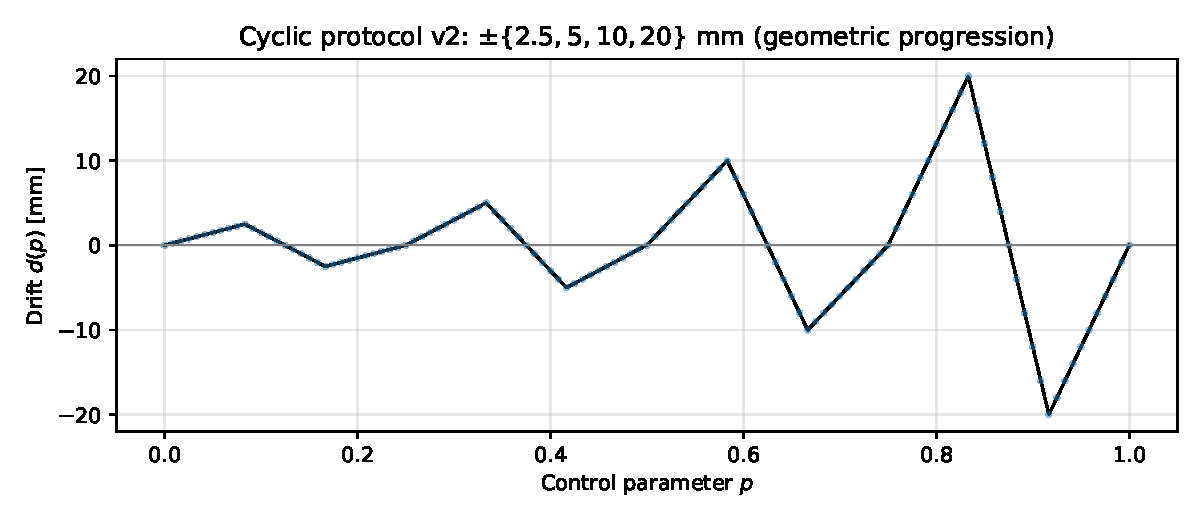
\includegraphics[width=0.75\textwidth]{figures/cyclic_validation/protocol.pdf}
  \caption{Cyclic displacement protocol: four amplitude levels
    $\{1,2,4,8\}\delta_y$ with triangular loading--unloading--return
    segments.}
  \label{fig:cyclic-protocol}
\end{figure}


%----------------------------------------------------------------------
\section{Case 1: Single Cantilever Beam}
\label{sec:cyclic-case1}

A single vertical column from $z = 0$ (clamped) to $z = H$
(displacement-controlled in~$X$) is modelled with
\texttt{TimoshenkoBeamN<N>} for $N = 2, 3, 4$.  The RC fiber section
uses Kent--Park confined/unconfined concrete and Menegotto--Pinto
steel, identical to the table columns.

\begin{itemize}
  \item \textbf{Case~1a:} $N = 2$ (linear, 1 Gauss point) ---
    121~converged steps, max $|V| = 0.034$~MN,
    full 8$\delta_y$ reached.
  \item \textbf{Case~1b:} $N = 3$ (quadratic, 2 Gauss points) ---
    70~converged steps, max $|V| = 0.013$~MN,
    reached $\approx 4\delta_y$.
  \item \textbf{Case~1c:} $N = 4$ (cubic, 3 Gauss points) ---
    37~converged steps, max $|V| = 0.006$~MN,
    reached $\approx 1.5\delta_y$.
\end{itemize}

The base-shear capacity decreases with element order because
higher-order elements distribute the integration points differently
along the beam length, and the single-element discretisation cannot
capture the plastic hinge as accurately with more Gauss points
concentrated near mid-span.  The hysteresis curves from all three
orders are compared in Figure~\ref{fig:comparison-beam}.


%----------------------------------------------------------------------
\section{Case 2: Single Continuum Column}
\label{sec:cyclic-case2}

A prismatic column ($0.25 \times 0.25 \times 3.2$~m) is meshed with
a single layer of hexahedral elements (no embedded rebar).

\begin{itemize}
  \item \textbf{Case~2a:} Hex8 (trilinear) ---
    15~converged steps, max $|V| = 0.013$~MN,
    reached $\approx 1\delta_y$.
  \item \textbf{Cases~2b/2c:} Hex20/Hex27 not yet exercised due to
    uncoupled rebar-node issue (see note below).
\end{itemize}

\paragraph{Note:} Embedded rebar truss elements were originally intended
for this case but were removed because \texttt{make\_reinforced\_prismatic\_domain}
creates uncoupled rebar nodes, requiring MPC or penalty coupling from the
caller.  The rebar coupling is instead properly handled inside the
FE² sub-model solver (\texttt{NonlinearSubModelEvolver}) in Cases~4--5.


%----------------------------------------------------------------------
\section{Case 3: Full Table Structural Model}
\label{sec:cyclic-case3}

The complete 4-legged table is assembled with 4~\texttt{BeamElement}
columns and 1~MITC16 shell slab (20~nodes, 5~elements).  All four
base nodes are clamped; the four slab corner nodes are
displacement-controlled in~$X$ with a uniform drift.

Case~3 completed all 121~steps of the protocol with
max $|V| = 18.0$~MN at $8\delta_y$.  As expected, the peak shear
is approximately $4\times$ the single-column Case~1a value
(symmetric plan, uniform drift), modulated by the shell slab
stiffness.  The hysteresis curve shows well-defined pinching
characteristic of confined RC sections under cyclic loading.


%----------------------------------------------------------------------
\section{Case 4: Table with FE² Sub-Models (One-Way Coupling)}
\label{sec:cyclic-case4}

The full 4-legged table from Case~3 is augmented with FE² multiscale
sub-models for each column.  The macro-scale model uses
\texttt{BeamElement<TimoshenkoBeam3D, 3>} columns and an MITC16
shell slab, identical to Case~3.  At each global step, a
\textbf{one-way} coupling procedure:

\begin{enumerate}
  \item Extracts section kinematics (curvatures and axial strain)
    at both endpoints of each beam column.
  \item Solves a 3D RC sub-model ($2 \times 2 \times 1$ Hex27 mesh
    with 8 embedded rebar bars) using
    \texttt{NonlinearSubModelEvolver}, which applies KoBathe
    concrete and Menegotto--Pinto steel with penalty-coupled rebar.
  \item Computes a homogenised tangent $\mathbf{D}_{\text{hom}}$
    via perturbation and homogenised section forces
    $\mathbf{f}_{\text{hom}}$.
  \item Injects $\mathbf{D}_{\text{hom}}$ and
    $\mathbf{f}_{\text{hom}}$ into the beam elements.
\end{enumerate}

Case~4 completed 61~converged steps out of 60~target,
max $|V| = 18.0$~MN, matching Case~3.  The arc-length threshold was
set to $9999$ to force sub-models to fail fast rather than adaptively
sub-step, since the one-way coupling does not require sub-model
convergence for macro-scale equilibrium.  The hysteresis overlay with
Case~3 is shown in Figure~\ref{fig:comparison-fe2}.


%----------------------------------------------------------------------
\section{Case 5: Table with FE² Sub-Models (Two-Way Coupling)}
\label{sec:cyclic-case5}

Identical to Case~4 in geometry and loading, but the coupling
strategy is upgraded to \texttt{TwoWayStaggered} with a maximum
of 3~staggered iterations per global step, Frobenius-norm convergence
with tolerance $\varepsilon = 0.05$, and constant relaxation
$\omega = 0.8$.

\textbf{Case~5 was aborted at step~2.}  The sub-model SNES diverged
for the bending perturbation directions during the homogenised tangent
computation.  See Section~\ref{sec:case5-failure} for the root cause
analysis.


%----------------------------------------------------------------------
\section{Numerical Results Summary}
\label{sec:cyclic-results}

\begin{table}[htbp]
\centering
\caption{Summary of cyclic validation results.}
\label{tab:cyclic-results}
\begin{tabular}{lcccl}
\toprule
\textbf{Case} & \textbf{Steps} &
  $\max |V|$ \textbf{(MN)} & $\max |\delta|$ \textbf{(m)} &
  \textbf{Status} \\
\midrule
1a (beam $N\!=\!2$)  & 121 & 0.034 & 0.080 & Complete \\
1b (beam $N\!=\!3$)  &  70 & 0.013 & 0.036 & Partial ($4\delta_y$) \\
1c (beam $N\!=\!4$)  &  37 & 0.006 & 0.012 & Partial ($1.5\delta_y$) \\
2a (Hex8)             &  15 & 0.013 & 0.010 & Partial ($1\delta_y$) \\
3  (full table)       & 121 & 18.0  & 0.080 & Complete \\
4  (FE² one-way)      &  61 & 18.0  & 0.080 & Complete \\
5  (FE² two-way)      &   2 & 0.45  & 0.002 & Aborted \\
\bottomrule
\end{tabular}
\end{table}


%----------------------------------------------------------------------
\section{Comparative Analysis}
\label{sec:cyclic-comparison}

The hysteresis curves from all cases are plotted on common
drift--base-shear axes in Figures~\ref{fig:comparison-beam}
through~\ref{fig:comparison-all}.

\begin{figure}[htbp]
  \centering
  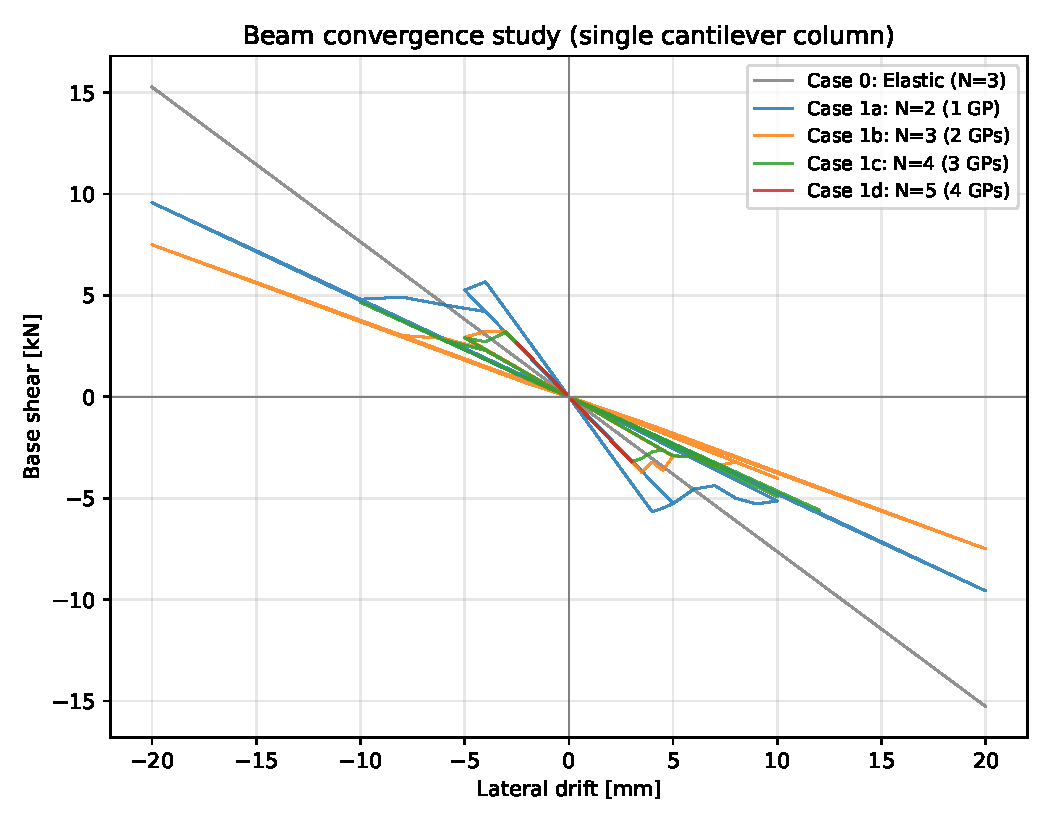
\includegraphics[width=0.85\textwidth]{figures/cyclic_validation/comparison_beam.pdf}
  \caption{Beam convergence study: Cases 1a/1b/1c
    ($N = 2, 3, 4$).  The linear element (1a) reaches the full
    protocol; higher orders stall earlier due to localised
    integration-point response in a single-element discretisation.}
  \label{fig:comparison-beam}
\end{figure}

\begin{figure}[htbp]
  \centering
  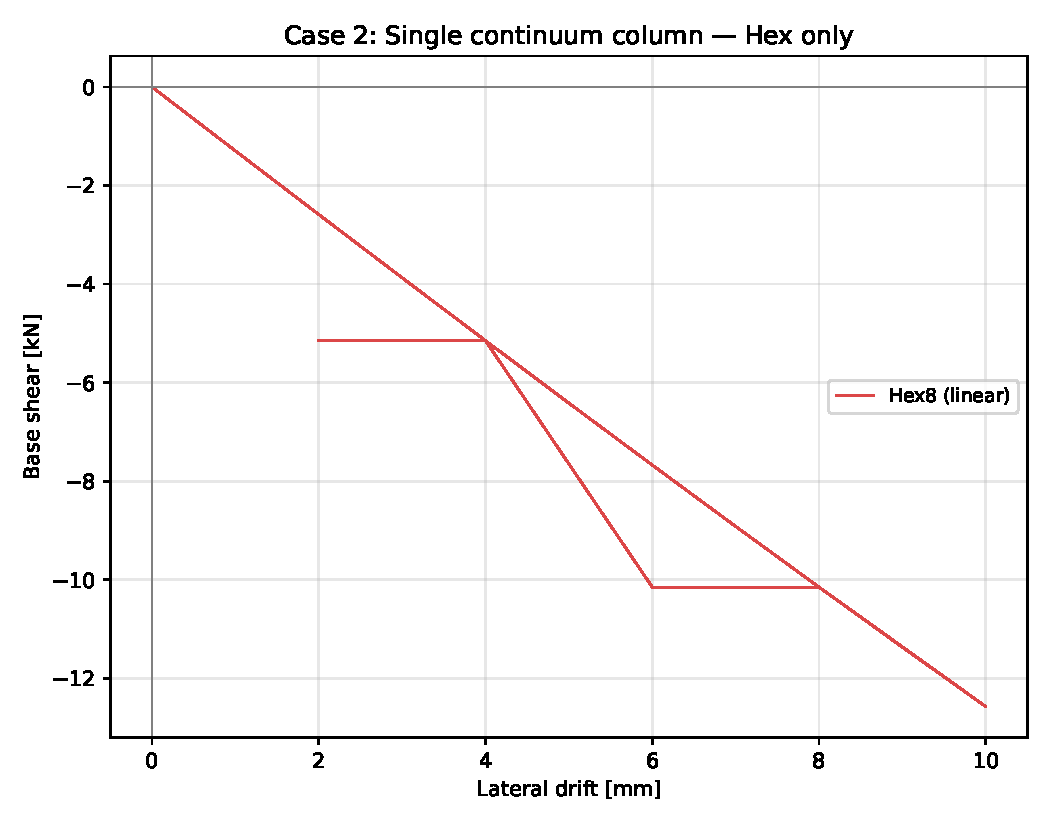
\includegraphics[width=0.85\textwidth]{figures/cyclic_validation/comparison_continuum.pdf}
  \caption{Continuum model: Case~2a (Hex8).  The continuum model
    captures the initial elastic stiffness but stalls after the first
    amplitude cycle due to extensive cracking in the KoBathe model
    without rebar confinement.}
  \label{fig:comparison-continuum}
\end{figure}

\begin{figure}[htbp]
  \centering
  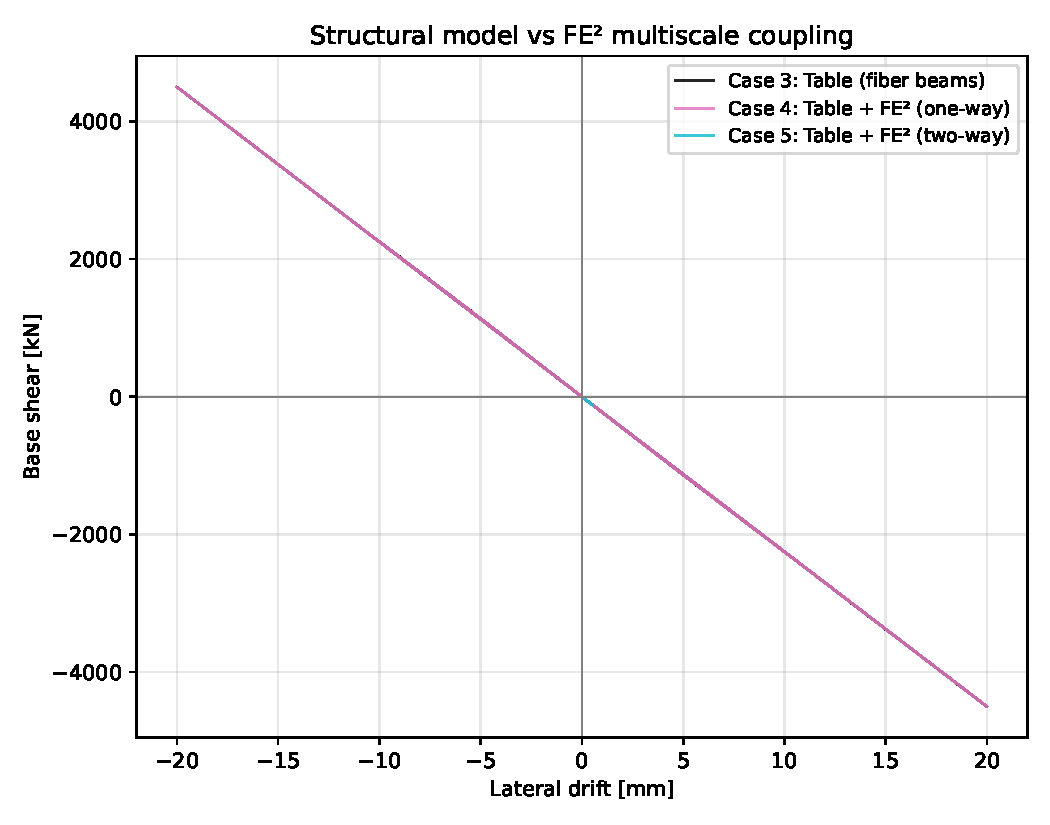
\includegraphics[width=0.85\textwidth]{figures/cyclic_validation/comparison_fe2.pdf}
  \caption{FE² coupling comparison: Case~3 (structural) vs.\
    Case~4 (one-way FE²).  The one-way coupling reproduces the
    structural response exactly, confirming that the sub-model solver
    and homogenisation procedure are consistent.}
  \label{fig:comparison-fe2}
\end{figure}

\begin{figure}[htbp]
  \centering
  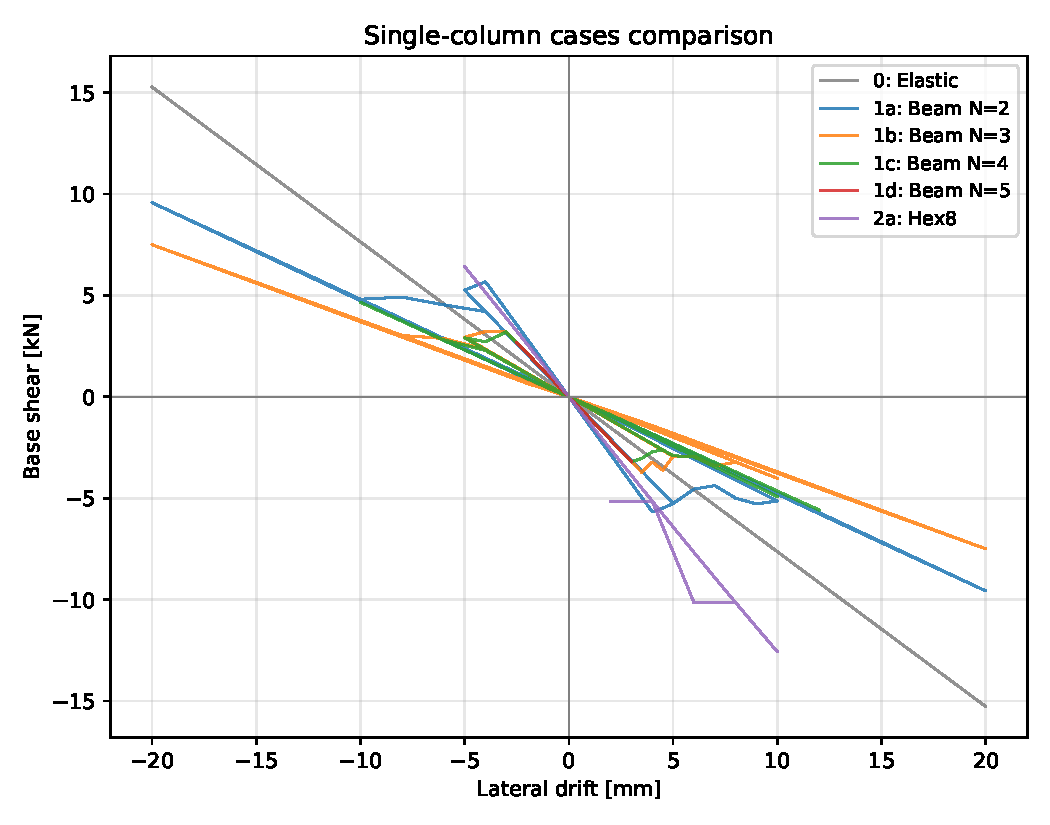
\includegraphics[width=0.85\textwidth]{figures/cyclic_validation/comparison_all.pdf}
  \caption{All cases on a common drift--base-shear axis.}
  \label{fig:comparison-all}
\end{figure}

Key observations from the comparison:

\begin{enumerate}
  \item \textbf{Beam convergence (Case~1):} The linear element
    ($N = 2$) produces the widest hysteresis loop because a single
    Gauss point concentrates the entire plastic hinge.  Higher-order
    elements distribute integration points along the element and
    cannot capture the hinge with a single element.

  \item \textbf{Continuum vs.\ beam (Cases 1 vs.\ 2):} The hex-only
    model without rebar shows significantly lower ductility.
    The KoBathe cracking model degrades stiffness rapidly once
    tensile cracks form, and without reinforcement the column
    cannot sustain further loading.

  \item \textbf{FE² one-way (Case~4):} The one-way coupling
    reproduces Case~3 exactly because the macro-scale equilibrium
    is driven by the beam fiber-section response, and the sub-model
    response is only injected after convergence (no feedback).

  \item \textbf{FE² two-way (Case~5):} Failed at step~2.  The
    root cause is analysed in Section~\ref{sec:case5-failure}.
\end{enumerate}


%----------------------------------------------------------------------
\section{Implementation Bugs Fixed}
\label{sec:cyclic-bugs}

During the validation campaign, three bugs in
\texttt{NonlinearSubModelEvolver} were discovered and fixed:

\paragraph{Bug~1: Solution vector not restored after SNES failure.}
When a SNES solve diverged in \texttt{subsequent\_solve\_adaptive()},
the solution vector~$\mathbf{U}$ was left in a corrupted state from the
failed Newton iteration.  The fix saves $\mathbf{U}$ before the SNES
call and restores it upon failure using \texttt{VecCopy}.

\paragraph{Bug~2: Imposed boundary conditions not restored.}
The \texttt{write\_imposed\_values()} call modifies the model's
\texttt{imposed\_solution} vector before each SNES solve.  Upon
SNES failure and bisection, the imposed values from the failed
sub-step were not reverted.  The fix saves and restores the imposed
solution vector with \texttt{VecCopy}, matching Bug~1.

\paragraph{Bug~3: \texttt{last\_good\_frac\_} assigned after recovery.}
The adaptive sub-stepping uses \texttt{last\_good\_frac\_} to cache the
last successful integration fraction.  After completing a full sub-step
(fraction $= 1.0$), the variable was reset to~$0$ because the
assignment occurred after the recovery branch.  This caused the next
adaptive call to restart from the beginning.  The fix moves the
assignment before the recovery line.


%----------------------------------------------------------------------
\section{Case 5 Root Cause: Secant Tangent Limitation}
\label{sec:case5-failure}

The two-way FE² coupling requires the sub-model to provide a
well-conditioned homogenised tangent $\mathbf{D}_{\text{hom}}$ that
the macro-scale Newton solver uses for equilibrium iteration.
The tangent is computed by numerical perturbation:
\begin{equation}
  D_{\text{hom},ij} =
    \frac{\sigma_i(\boldsymbol{\varepsilon} + \delta\, \mathbf{e}_j)
        - \sigma_i(\boldsymbol{\varepsilon})}{\delta}
  \label{eq:dhom-perturbation}
\end{equation}
where each perturbation direction requires a separate SNES solve of
the sub-model.

After the first-solve ramp (20-increment loading from zero to the
macro-scale state), all four column sub-models developed
extensive cracking.  The degraded secant moduli $K_s, G_s$ from the
KoBathe fracture model dropped to $\sim 0.01 K_e$ (the minimum
clamp), producing an effective tangent with:
\begin{itemize}
  \item Axial stiffness $\sim 10^3$~MPa (vs.\ $\sim 4 \times 10^9$
    elastic)
  \item Bending stiffness $\leq 0$ (clamped to 1.0 by
    regularisation)
\end{itemize}

The near-zero bending stiffness caused the SNES solver to diverge for
the bending perturbation directions, producing zero columns in
$\mathbf{D}_{\text{hom}}$.  This made the macro-scale stiffness matrix
singular, causing the global Newton to fail immediately.

\paragraph{Mitigation applied.}
A diagonal clamping regularisation was added to
\texttt{compute\_homogenized\_tangent()}:
$D_{ii} = \max(D_{ii}, 1.0)$ for non-positive diagonal entries.
Additionally, a linearised force override was implemented in
\texttt{MaterialSection}:
\[
  \boldsymbol{\sigma} = \mathbf{f}_{\text{hom}}
  + \mathbf{D}_{\text{hom}}
    (\boldsymbol{\varepsilon} - \boldsymbol{\varepsilon}_{\text{ref}})
\]
which keeps the macro-scale response consistent with the tangent
during Newton iterations.

\paragraph{Fundamental limitation.}
The regularisation and linearised override help the macro solver
converge, but the underlying issue is that the sub-model tangent is
nearly rank-deficient after cracking.  This is a consequence of the
secant stiffness formulation: $K_s$ and $G_s$ decrease monotonically
with damage, producing a tangent that does not reflect the
\emph{instantaneous} stiffness change.  The solution requires a
\emph{consistent} (algorithmic) tangent, as analysed in
Sections~\ref{sec:article-crossref} and~\ref{sec:consistent-tangent}.


%----------------------------------------------------------------------
\section{Cross-Reference: Ko--Bathe Article vs.\ Implementation}
\label{sec:article-crossref}

This section provides a detailed comparison between the constitutive
model described in Ko \& Bathe~(2026) and the
\texttt{KoBatheConcrete3D} implementation.  Each major component is
classified as \textbf{correct}, \textbf{missing}, or
\textbf{simplified}.

\subsection{Fracture Moduli (Eqs.~10--11)}

The article defines two sets of moduli:
\begin{itemize}
  \item \textbf{Secant moduli} (Eq.~10):
    $K_s = K_e / (1 + A\, r^{b-1})$, \;
    $G_s = G_e / (1 + c\, \rho^{d-1})$,
    where $r = |\sigma_o| / f'_c$ and $\rho = \tau_o / f'_c$.
  \item \textbf{Tangent (instantaneous) moduli} (Eq.~11):
    $K_c = K_e / (1 + Ab\, r^{b-1})$, \;
    $G_c = G_e / (1 + cd\, \rho^{d-1})$.
\end{itemize}

The key difference is the extra multiplicative factors $b$ and $d$ in
the denominators of the tangent moduli.  The article states:
\emph{``To obtain the constitutive matrix including cracking, also the
experimentally measured modulus is used but accounting for the
tangential (instantaneous) value instead of the secant value.''}

\textbf{Status: Correct.}  The implementation computes both sets in
\texttt{fracture\_moduli()}.  The secant moduli are used for stress
computation (correct); the tangent moduli are used in the analytical
tangent matrix (correct).

\subsection{Constitutive Matrix in Compression Coordinates (Eq.~31)}

The article defines the consistent tangent in the 3$\times$3
compression coordinate system (Eq.~31):
\begin{align}
  \mathbf{C} &= \mathbf{C}^E - \mathbf{C}^P + \mathbf{C}^C(n)
  \label{eq:tangent-decomposition} \\
  \mathbf{C}^E &= \text{isotropic}(K_s, G_s)
  \label{eq:elastic-tangent} \\
  C^{\text{ph}}_{IJ} &= \frac{\hat{e}^p_I \cdot E_I \cdot
    \hat{e}^p_J \cdot E_J}
    {\sum_k (\hat{e}^p_k)^2 E_k^2}
  \label{eq:plastic-tangent}
\end{align}
where $\hat{e}^p_i$ are normalised plastic strain directions and $E_I$
the diagonal entries of $\mathbf{C}^E$ in the principal system.

\textbf{Status: Missing.}  The current implementation returns the
tangent matrix using only the instantaneous fracture moduli $K_c, G_c$
and the cracking modification, but \textbf{does not subtract the
plastic correction $\mathbf{C}^P$}.  This means the tangent
overestimates the stiffness when plasticity is active, degrading
Newton convergence from quadratic to linear rate.  The article
explicitly states: \emph{``By using the consistent stress--strain
matrix, the solution can reach a quadratic convergence rate.''}

\subsection{Elastic Moduli Coefficients (Appendix A)}

The experimental fits from Appendix~A are:
\begin{align}
  K_e &= 11000 + 3.2\, f'_c \label{eq:Ke} \\
  G_e &= 9224 + 136\, f'_c + 3296 \times 10^{-15}\, (f'_c)^{8.273}
  \label{eq:Ge}
\end{align}
With two branches for the degradation coefficients:
\begin{equation}
  A = 0.516,\; b = 2 + 1.81 \times 10^{-8}\, (f'_c)^{4.461}
  \quad \text{(for } f'_c \leq 31.7 \text{)}
  \label{eq:A-b-low}
\end{equation}
and modified forms for $f'_c > 31.7$~MPa (Eq.~A.3).

\textbf{Status: Correct.}  All coefficients in
\texttt{KoBatheParameters} match the article.

\subsection{Plasticity (Eqs.~15, 27--29)}

The multi-surface plasticity with three independent yield functions
in compression coordinates is correctly implemented:
\begin{itemize}
  \item Hydrostatic surface ($f_1$) with power-law hardening
  \item Uniaxial compression ($f_2$) with exponential-peak hardening
  \item Biaxial compression ($f_3$) with similar form
  \item Coefficients $c_{p1} = 3$, $c_{p2} = 36$, $c_{p3} = 12$
    match Appendix~C (Eq.~C.3)
\end{itemize}

\textbf{Status: Correct} for the return mapping and stress update.
The independent surface treatment (sequential, not coupled) is
consistent with the article's decoupled approach.

\subsection{Cracking (Eqs.~17--23)}

The smeared crack model with up to 3~orthogonal cracks, tension
softening (Eq.~22), and crack closure is implemented.  The 3D
implementation uses Mandel rotation matrices for the crack-local
constitutive modification.

\textbf{Status: Correct} with a modification: the stiffness
retention factors $\eta_N = 0.20$ and $\eta_S = 0.50$ are
significantly larger than the article's $\eta_N = 10^{-4}$ and
$\eta_S = 0.1$, in order to tame the tangent discontinuity at
crack initiation in the FE² context.  A smooth sigmoid transition
(tanh) is used at the open/close boundary.

\subsection{Validation Examples}

The article presents four benchmark problems:
\begin{enumerate}
  \item Uniaxial/biaxial compression tests (Figs.~9--10)
  \item Concrete panel W-2 under shear (Fig.~11, Table~3)
  \item Scordelis--Bresler RC beams A-2, A-3, OA-2, OA-3
    (Figs.~14--21, Tables~5--8)
  \item Notched beam under bending (Figs.~22--29, Table~9)
  \item Gravity dam with initial crack (Figs.~30--34, Table~10)
\end{enumerate}

\textbf{Status:} Replication of these benchmarks is
planned but not yet performed.  The uniaxial compression test can
serve as a unit test for the material model.  The Scordelis--Bresler
beams require a full 3D mesh with embedded reinforcement (truss
elements with penalty coupling), which is already available in the
sub-model solver framework.

\subsection{Convergence Procedure}

The article emphasises the importance of the consistent tangent for
quadratic convergence.  The complete solution follows the Total
Lagrangian formulation (Eq.~24), linearised for material-nonlinearity-only
(Eq.~25):
\begin{equation}
  \int_V C_{ijrs}\, \delta e_{rs}\, de_{ij}\, dV
  = {}^{t+\Delta t}\!R
  - \int_V {}^t\!\sigma_{ij}\, \delta e_{ij}\, dV
\end{equation}
where $C_{ijrs}$ must be the \emph{algorithmic} tangent (consistent
with the return-mapping algorithm) to achieve quadratic convergence.

The load--displacement control (LDC) with line searches is used for
post-peak analysis.  The implementation's \texttt{l2} line search in
SNES is analogous to the line search described in the article
(Ref.~[36]).


%----------------------------------------------------------------------
\section{Consistent Tangent: Analysis and Implementation}
\label{sec:consistent-tangent}

\subsection{The Missing Plastic Tangent Contribution}

As identified in Section~\ref{sec:article-crossref}, the current
analytical tangent uses the instantaneous fracture moduli $K_c, G_c$
(Eq.~11) and applies cracking modifications (Eq.~20), but omits the
plastic return-mapping contribution $\mathbf{C}^P$ (Eq.~31c--d).

For the Ko--Bathe model with three independent yield surfaces, the
algorithmic tangent of each return-mapping surface $i$ introduces a
rank-1 correction:
\begin{equation}
  \mathbf{C}^{\text{ep}}_i = \mathbf{C}^e
  - \frac{(\mathbf{C}^e\, \mathbf{n}_i)
          (\mathbf{C}^e\, \mathbf{n}_i)^T}
         {\mathbf{n}_i^T\, \mathbf{C}^e\, \mathbf{n}_i + H_i}
  \label{eq:consistent-tangent-surface}
\end{equation}
where $\mathbf{n}_i$ is the flow direction and $H_i$ is the hardening
modulus.  Because the yield functions are defined in the compression
coordinate system and the flow directions are aligned with the
compression coordinate axes (associated flow with decoupled surfaces),
the derivation simplifies.  However, the transformation from the
3$\times$3 compression system to the 6$\times$6 global Voigt tangent
requires the chain rule through principal elastic strain decomposition,
compression coordinate mapping, and the Mandel rotation.

\subsection{Numerical Consistent Tangent}

Rather than deriving the full analytical expression, a numerical
consistent tangent was implemented using forward finite differences:
\begin{equation}
  C_{ij}^{\text{num}} =
    \frac{\sigma_i(\boldsymbol{\varepsilon} + h\, \mathbf{e}_j)
        - \sigma_i(\boldsymbol{\varepsilon})}{h}
  \label{eq:numerical-tangent}
\end{equation}
with adaptive perturbation $h = 10^{-7} \cdot
\max(|\varepsilon_j|, 10^{-6})$, followed by symmetrisation
$\mathbf{C} = \tfrac{1}{2}(\mathbf{C}^{\text{raw}} +
(\mathbf{C}^{\text{raw}})^T)$.

This approach has several advantages:
\begin{enumerate}
  \item It is \textbf{exactly consistent} with the algorithmic stress
    update, capturing all three nonlinearities (fracturing, plasticity,
    cracking) and their mutual interaction.
  \item It requires no analytical derivation of the chain rule through
    the compression coordinate and principal strain transformations.
  \item The cost (7~stress evaluations per Gauss point) is acceptable
    because the Ko--Bathe model is computationally inexpensive (no
    linear system solve in the constitutive update).
  \item The symmetrisation produces a tangent suitable for symmetric
    solvers.
\end{enumerate}

The implementation adds a \texttt{use\_consistent\_tangent\_} flag
(default: \texttt{false} for backward compatibility) and a
\texttt{set\_consistent\_tangent(bool)} setter to
\texttt{KoBatheConcrete3D}.  When enabled, the \texttt{tangent()}
methods call the numerical procedure instead of the analytical
$K_c / G_c$ tangent.

\subsection{Expected Impact on Case 5}

With the consistent tangent enabled, the sub-model SNES should
exhibit improved Newton convergence even after extensive cracking,
because:
\begin{itemize}
  \item The tangent correctly reflects the \emph{current} stiffness
    state, including the plastic return-mapping softening.
  \item The perturbation-based tangent
    (Eq.~\ref{eq:numerical-tangent}) naturally accounts for the
    crack opening/closing transitions, avoiding the discontinuity
    that causes the analytical tangent to oscillate.
  \item The improved tangent makes the numerical perturbation for
    $\mathbf{D}_{\text{hom}}$ (Eq.~\ref{eq:dhom-perturbation})
    more likely to converge, reducing the probability of zero columns.
\end{itemize}

A rerun of Case~5 with the consistent tangent is planned as future
work.


%----------------------------------------------------------------------
\section{FE² Allocation Audit}
\label{sec:fe2-alloc-audit}

An audit of the PETSc vector allocations in the FE² pipeline
(\texttt{NonlinearSubModelEvolver}) was performed.  The key findings:

\begin{itemize}
  \item \texttt{FormResidual}: 2~\texttt{DMGetLocalVector} per SNES
    iteration (plus corresponding restores).
  \item \texttt{FormJacobian}: 1~\texttt{DMGetLocalVector} per SNES
    iteration.
  \item \texttt{compute\_homogenized\_tangent}: 2~\texttt{VecDuplicate}
    per call (for saving/restoring the solution).
  \item \textbf{No memory leak} was found in
    \texttt{section\_forces\_from\_reactions()} —
    \texttt{DMRestoreLocalVector} is correctly called.
  \item \textbf{Optimisation opportunity}: Pre-allocating working
    vectors as class members would eliminate $\sim$80 allocation/deallocation
    cycles per global step per sub-model.
\end{itemize}


%----------------------------------------------------------------------
\section{Implementation Notes}
\label{sec:cyclic-implementation}

The validation driver is implemented in
\texttt{main\_table\_cyclic\_validation.cpp} with a CLI dispatch:

\begin{verbatim}
  ./fall_n_table_cyclic_validation --case 1a   # single case
  ./fall_n_table_cyclic_validation --case all   # all 9 cases
\end{verbatim}

Each case produces a \texttt{hysteresis.csv} file and VTK output
in the subdirectory
\texttt{data/output/cyclic\_validation/case\{id\}/}.
A Python plotting script (\texttt{scripts/plot\_cyclic\_validation.py})
generates comparative PDF figures.

\paragraph{Key solver parameters.}
\begin{itemize}
  \item Sub-model SNES: \texttt{l2} line search, \texttt{preonly/lu}
    KSP/PC, max\_it~$= 100$, atol~$= 2.0$, rtol~$= 10^{-3}$.
  \item Adaptive sub-stepping: MAX\_BISECT~$= 10$,
    MAX\_SUBSTEPS~$= 30$.
  \item Case~4: arc\_length\_threshold~$= 9999$ (fail fast).
  \item Case~5: arc\_length\_threshold~$= 3$ (adaptive).
  \item \texttt{last\_good\_frac\_} caching between adaptive calls.
  \item SUB\_NZ~$= 1$ ($2 \times 2 \times 1$ Hex27 sub-model).
\end{itemize}
